\section{Diskussion}
\label{sec:Diskussion}

\addsec{Anhang}
\label{sec:Anhang}

\begin{figure}
    \centering
    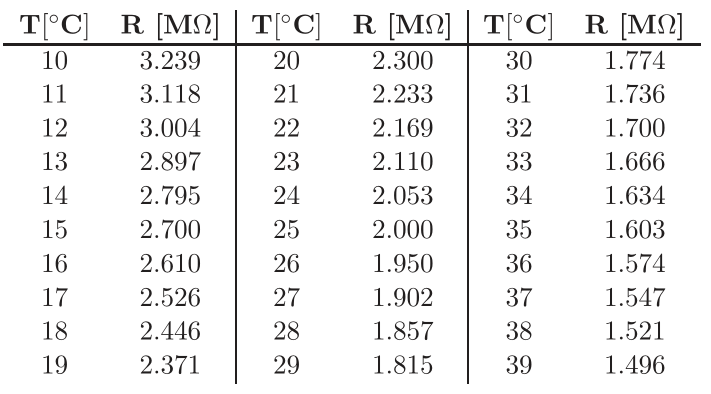
\includegraphics[width=0.7\textwidth]{bilder/thermistorwiderstand.png}
    \caption{Thermistor-Widerstandstabelle \cite{sample}.}
    \label{fig:thermistor}
\end{figure}

\begin{figure}
    \centering
    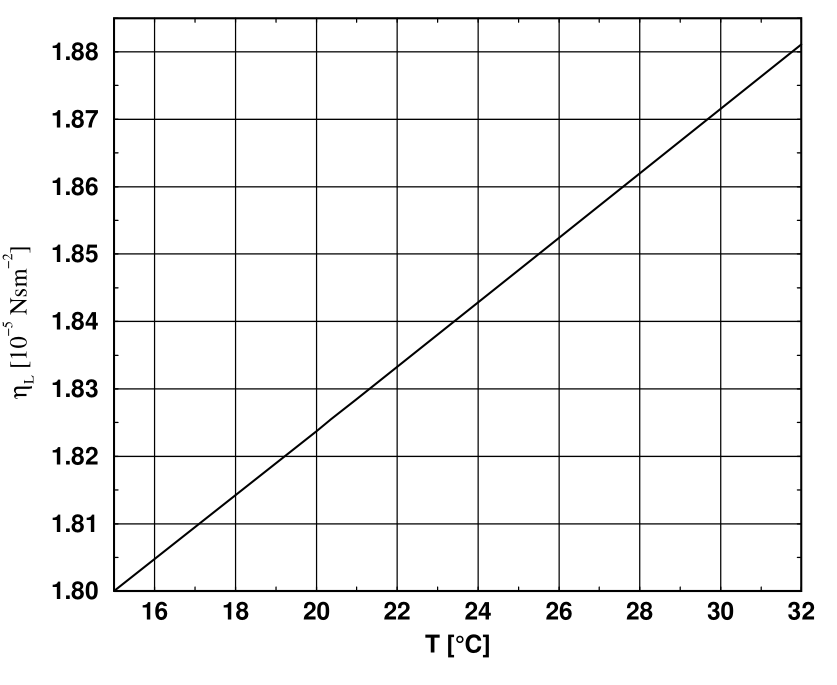
\includegraphics[width=0.7\textwidth]{bilder/viskositaet.png}
    \caption{Viskosität der Luft in Abhängigkeit der Temperatur \cite{sample}.}
    \label{fig:viskositaet}
\end{figure}

\begin{figure}
    \centering
    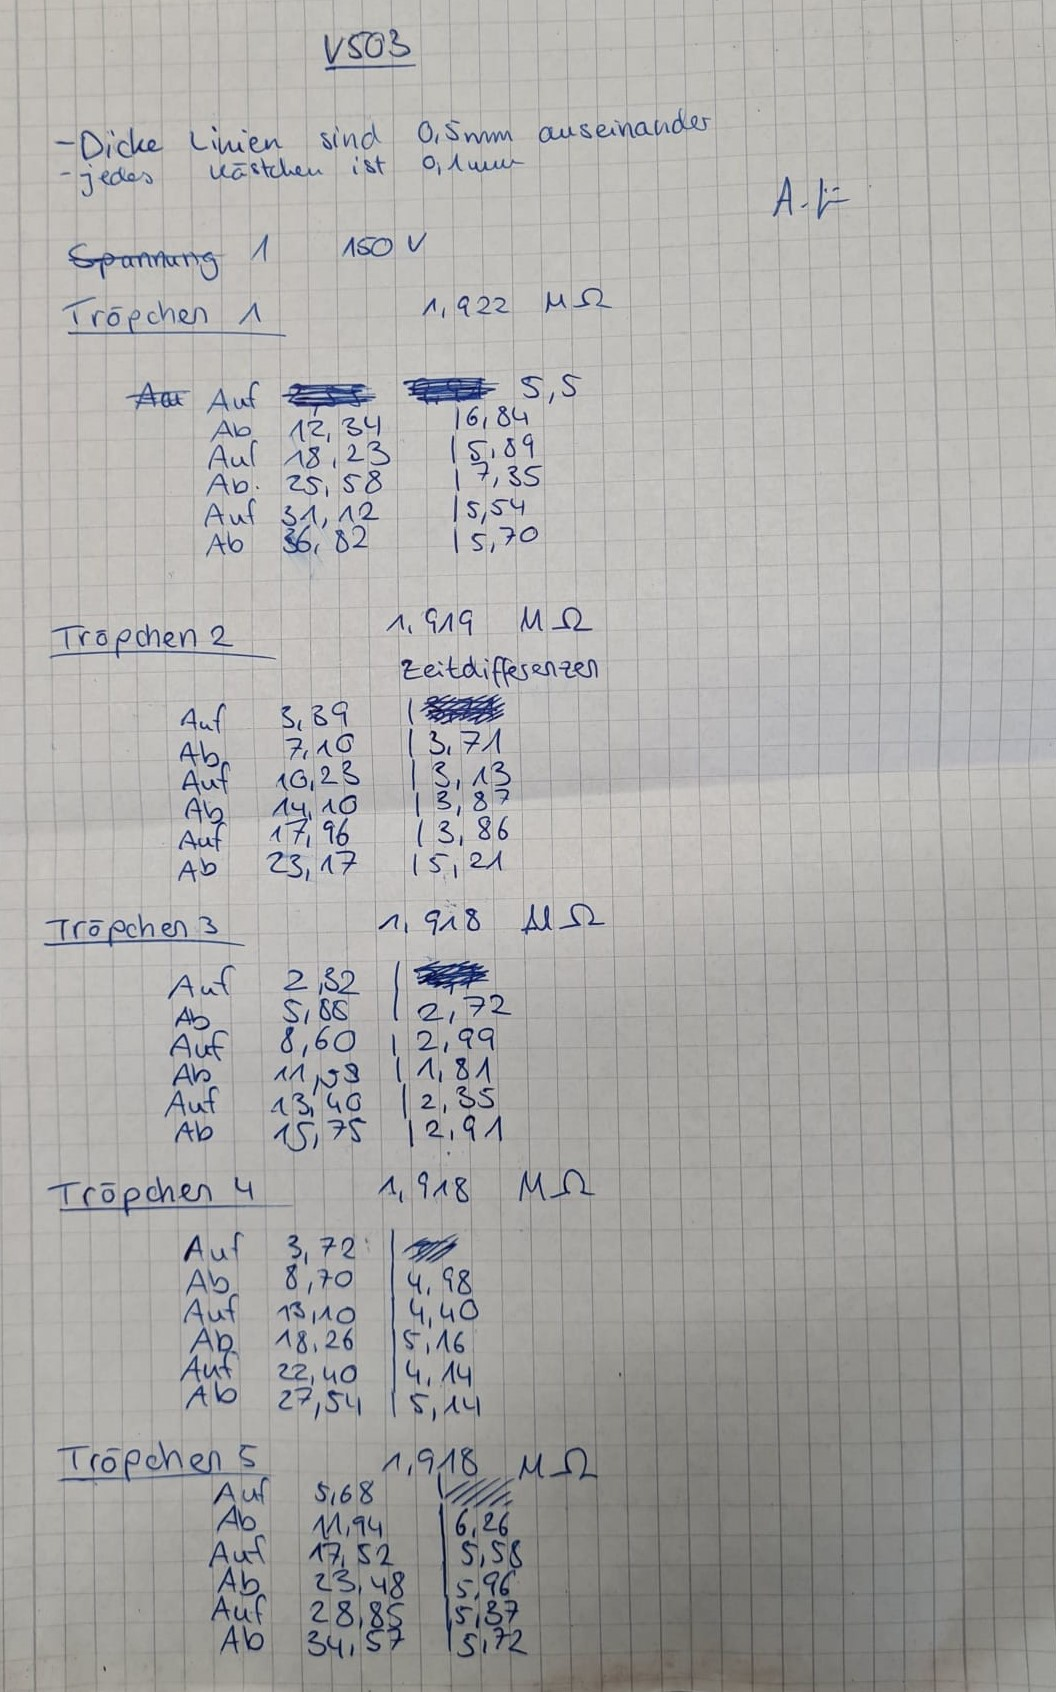
\includegraphics[width=0.7\textwidth]{bilder/Spannung1.jpg}
    \caption{Messwerte der ersten Spannung.}
\end{figure}

\begin{figure}
    \centering
    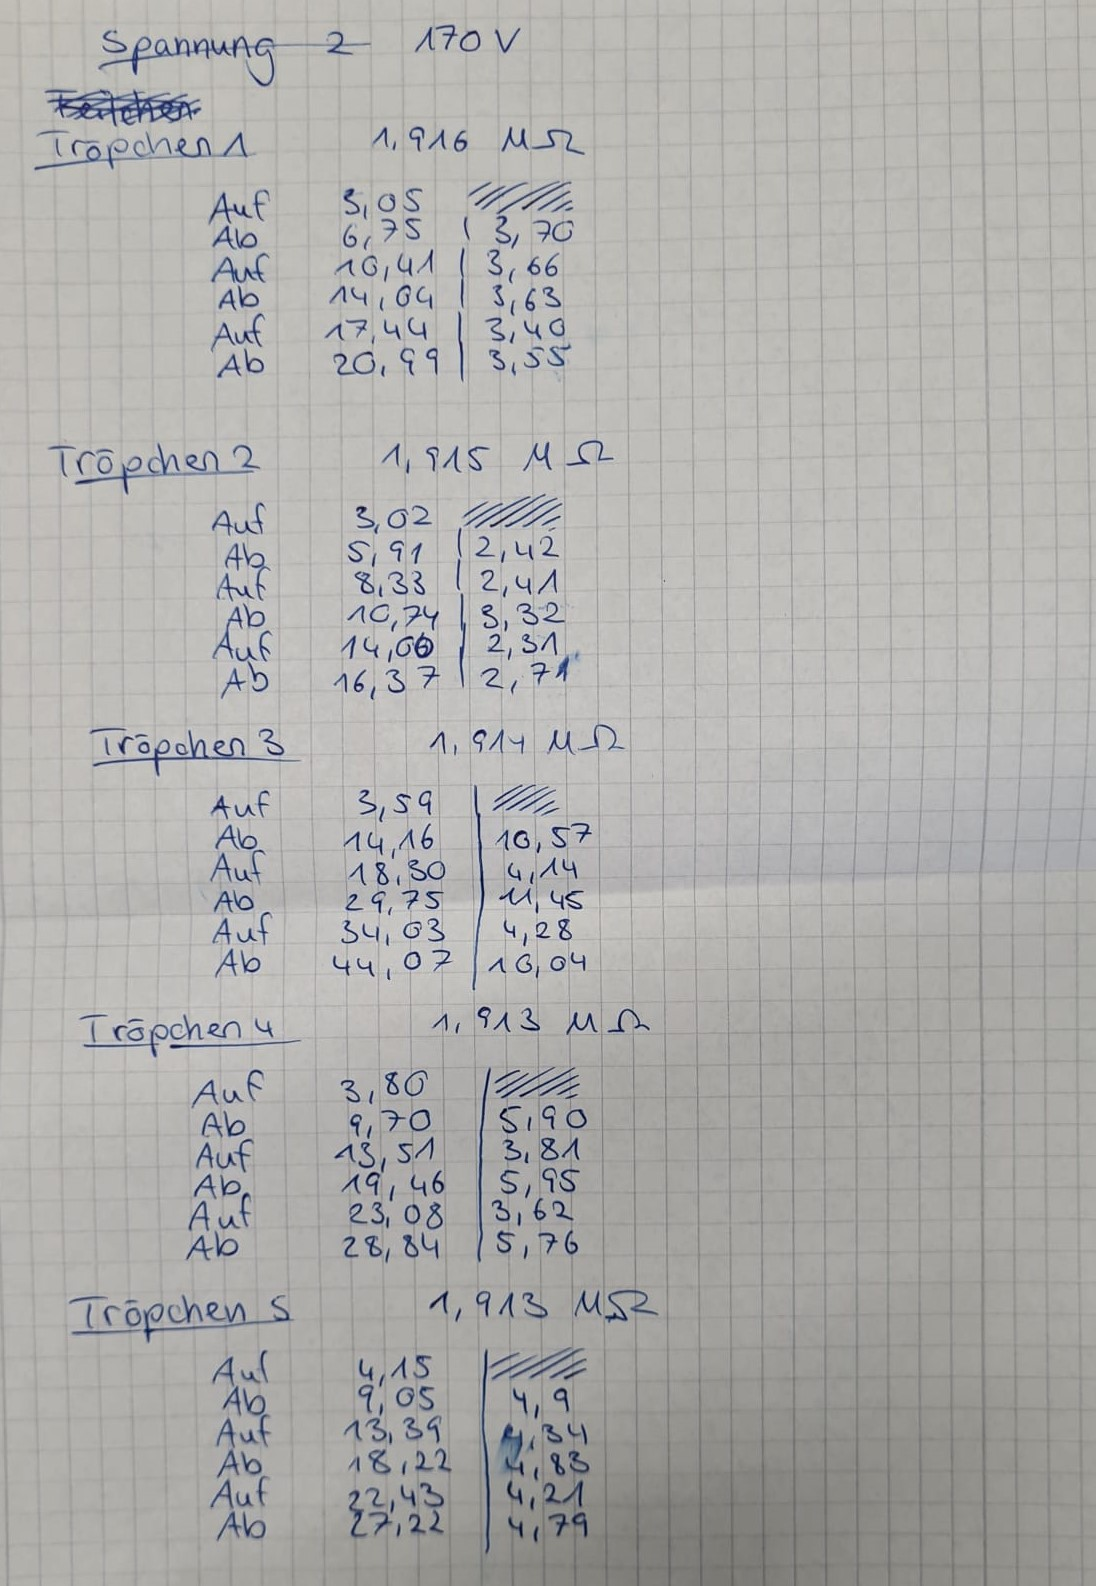
\includegraphics[width=0.7\textwidth]{bilder/Spannung2.jpg}
    \caption{Messwerte der zweiten Spannung.}
\end{figure}

\begin{figure}
    \centering
    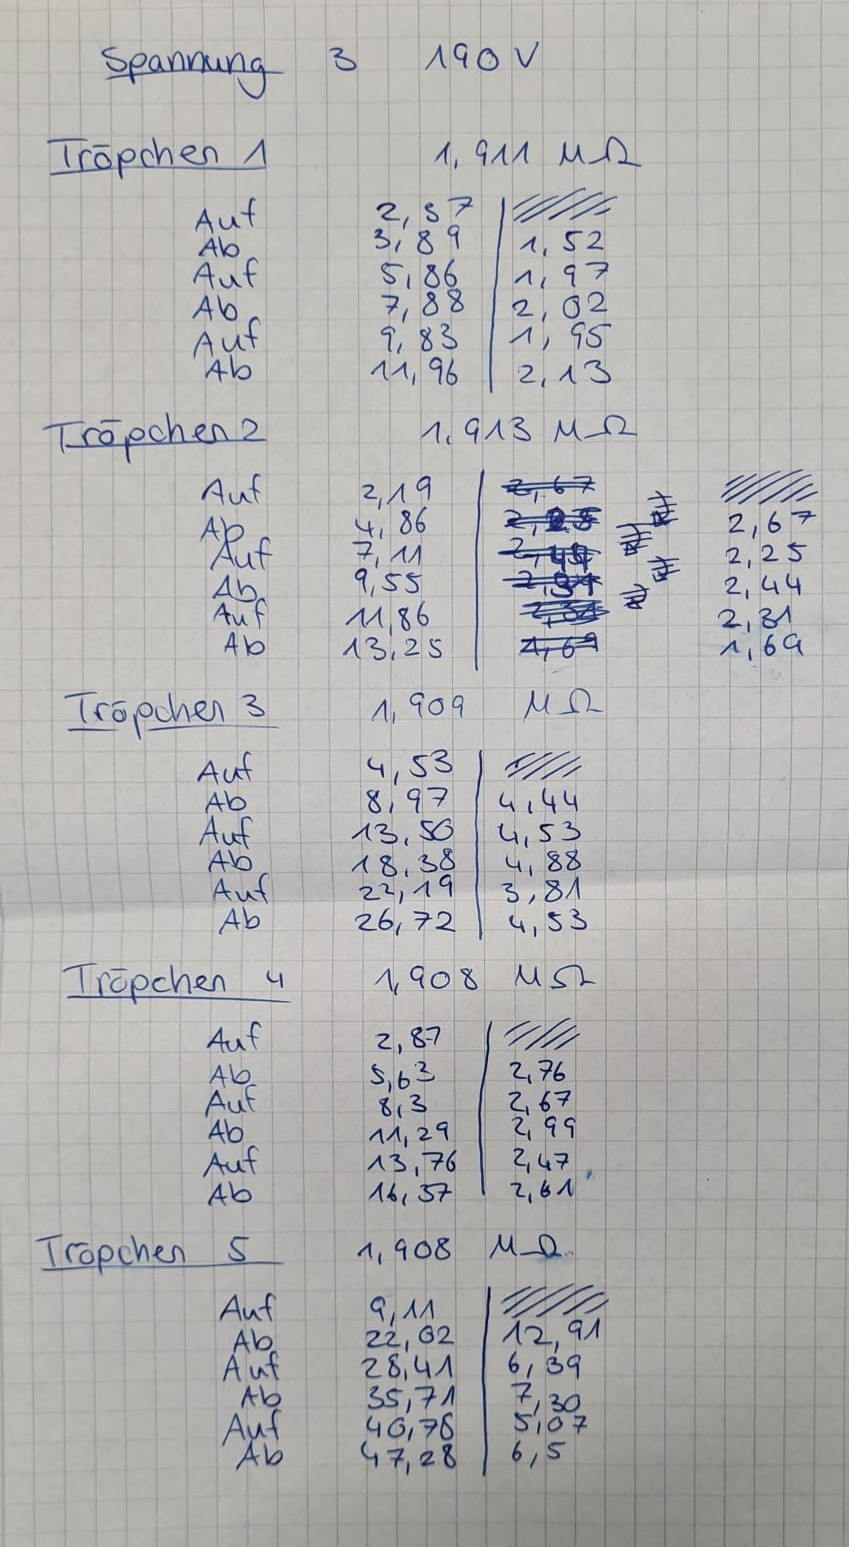
\includegraphics[width=0.7\textwidth]{bilder/Spannung3.jpg}
    \caption{Messwerte der dritten Spannung.}
\end{figure}

\begin{figure}
    \centering
    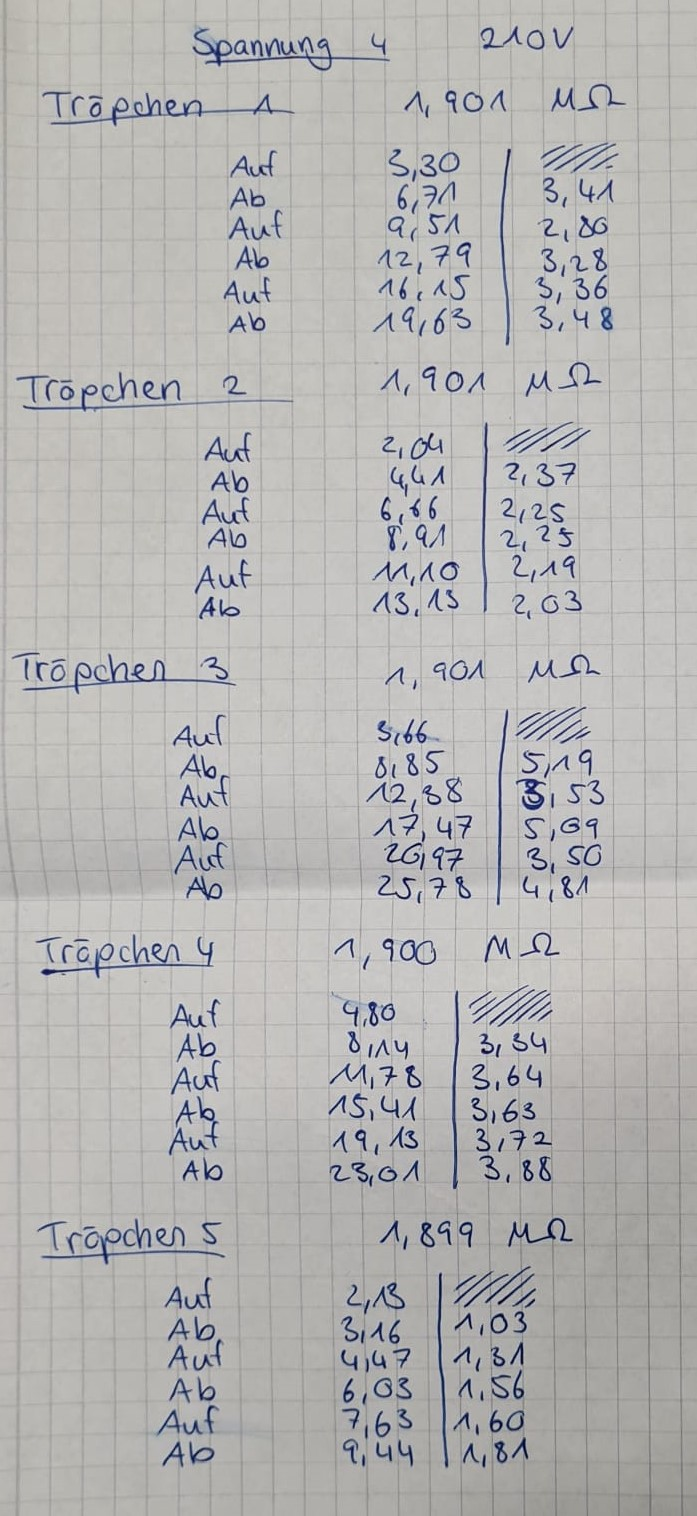
\includegraphics[width=0.7\textwidth]{bilder/Spannung4.jpg}
    \caption{Messwerte der vierten Spannung.}
\end{figure}

\begin{figure}
    \centering
    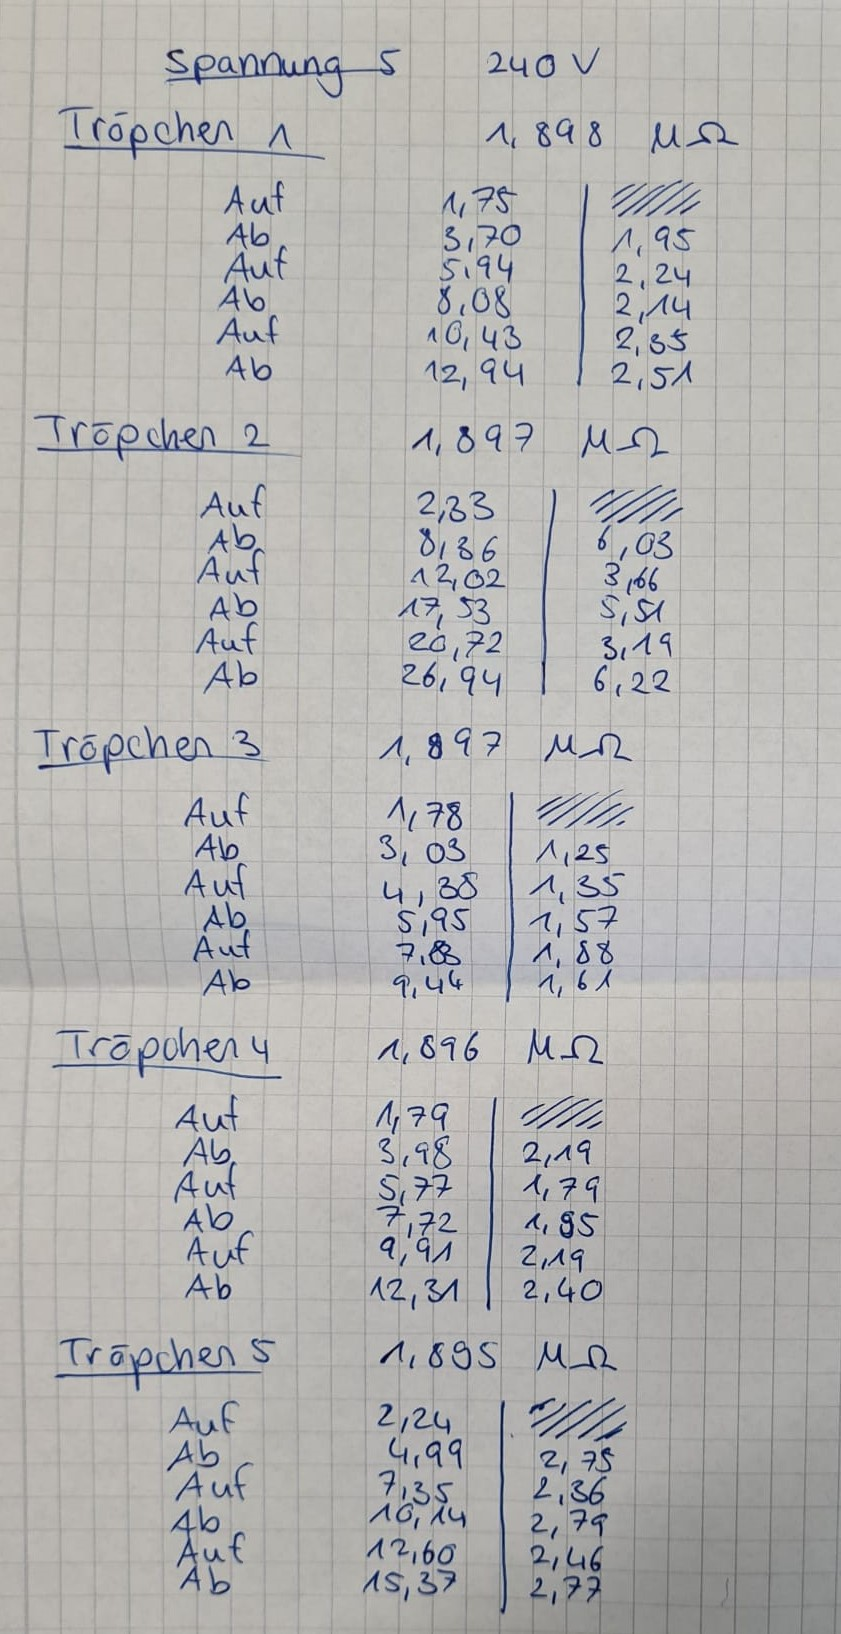
\includegraphics[width=0.7\textwidth]{bilder/Spannung5.jpg}
    \caption{Messwerte der fünften Spannung.}
\end{figure}